\documentclass[../../../interview-questions.tex]{subfiles}

\begin{document}

\subsection{细节基础问题}

Java获取Class的三种方法:

\begin{lstlisting}[language=Java]
Class<?> class = ClassName.class;
Class<?> class = Class.forName("类名全路径");
Class<?> class = object.getClass();
\end{lstlisting}


\paragraph{Java的BigDecimal如何解决浮点数精度问题}

BigDecimal的解决方案就是,不使用二进制,而是使用十进制(BigInteger)+小数点位置(scale)来表示小数.当使用BigDecimal来进行运算时,也就可以分解成两部分,BigInteger间的运算,以及小数点位置scale的更新.BigInteger可以表示任意精度的整数。当你使用long类型进行运算,可能会产生溢出时就要考虑使用BigInteger了。BigDecimal就使用了BigInteger作为backend。那么BigInteger是如何做到可以表示任意精度的整数的?答案是使用数组来表示。BigInteger存储大数的方式就是将数字存储在一个整型的数组中,这样就能解决可以存很多很多位数字的问题。那么,只用一个整型数组的话,如何表示一个整数的正负呢?那么就需要有一个单独的成员变量来标明该数的正负。

\begin{lstlisting}[language=Java]
public static void main(String[] args)  {
    byte[] mag = {
            2, 1 // 10 00000001 == 513
    };
    System.out.println(new BigInteger(mag));
}
\end{lstlisting}

下面看看BigInteger有哪些重点的属性,主要的有下面两个:

\begin{itemize}
    \item {\bf{final int signum}} signum属性是为了区分:正负数和0的标志位,整数用1表示,负数用-1表示,零用0表示。
    \item {\bf{final int[] mag}} mag是magnitude的缩写形式,mag数组是存储BigInteger数值大小的,采用big-endian的顺序,也就是高位字节存入低地址,低位字节存入高地址,依次排列的方式。
\end{itemize}

如何避免精度问题?在使用的时候,有两种方法:

使用new BigDecimal(String);
使用BigDecimal.valuOf(Double);

即先转成字符串再转成BigDecimal。BigDecimal.valueOf(double)其实就等同于new BigDecimal(String)。

\paragraph{Java栈溢出(StackOverflowError)}

递归调用方法如果递归的深度过深,就会出现栈溢出(StackOverflowError)异常。如果这个区域允许动态扩展,但是无法申请到足够的内存,也会出现栈溢出。调整栈溢出的大小Xss(Stack Size)。最简单的方法就是细致的检查stack trace,找出行号的重复模式。这些重复的行号代表了被递归调用的代码。确认递归实现没有问题,你可以通过-Xss参数增加栈的大小,这个参数可以在项目配置或命令行指定。

\paragraph{Java汇编}

查看汇编代码前,编译成class文件:

\begin{lstlisting}[language=Bash]
javac Bar.java
\end{lstlisting}

如下命令打印汇编指令:

\begin{lstlisting}[language=Bash]
java -Xcomp -XX:+UnlockDiagnosticVMOptions -XX:+PrintAssembly -Xcomp -XX:CompileCommand=dontinline,Demo.sum -XX:CompileCommand=compileonly,Demo.sum Demo
java -XX:+UnlockDiagnosticVMOptions -XX:+PrintAssembly Demo
\end{lstlisting}

汇编示例如下:
 
\begin{lstlisting}[language=Bash]
Loaded disassembler from /Library/Java/JavaVirtualMachines/jdk1.8.0_112.jdk/Contents/Home/jre/lib/hsdis-amd64.dylib
Decoding compiled method 0x00000001086484d0:
Code:
[Disassembling for mach='i386:x86-64']
[Entry Point]
[Constants]
  # {method} {0x0000000107847230} 'sum' '()V' in 'Bar'
  #           [sp+0x40]  (sp of caller)
  0x0000000108648620: mov    0x8(%rsi),%r10d
  0x0000000108648624: shl    $0x3,%r10
  0x0000000108648628: cmp    %rax,%r10
  0x000000010864862b: jne    0x0000000108584e20  ;   {runtime_call}
  0x0000000108648631: data32 data32 nopw 0x0(%rax,%rax,1)
  0x000000010864863c: data32 data32 xchg %ax,%ax
\end{lstlisting}



\paragraph{负载均衡(Load Balance)的原理}

从应用场景上来说,常见的负载均衡模型有全局负载均衡和集群内负载均衡,从产品形态角度来说,又可以分为硬件负载均衡和软件负载均衡。全局负载均衡一般通过DNS实现,通过将一个域名解析到不同VIP,来实现不同的region调度能力;硬件负载均衡器常见的有F5、A10、Array,它们的优缺点都比较明显,优点是功能强大,有专门的售后服务团队,性能比较好,缺点是缺少定制的灵活性,维护成本较高;现在的互联网更多的思路是通过软件负载均衡来实现,这样可以满足各种定制化需求,常见的软件负载均衡有 LVS、Nginx、Haproxy。系统的扩展可分为纵向(垂直)扩展和横向(水平)扩展。纵向扩展,是从单机的角度通过增加硬件处理能力,比如CPU处理能力,内存容量,磁盘等方面,实现服务器处理能力的提升,不能满足大型分布式系统(网站),大流量,高并发,海量数据的问题。因此需要采用横向扩展的方式,通过添加机器来满足大型网站服务的处理能力。

\subparagraph{轮询调度}

轮询调度(Round Robin Scheduling)算法\footnote{\url{https://blog.csdn.net/u012891504/article/details/53434704}}就是以轮询的方式依次将请求调度到不同的服务器,即每次调度执行i = (i + 1) mod n,并选出第i台服务器。通常取模运算也叫取余运算,它们返回结果都是余数。rem 和 mod 唯一的区别在于:当 x 和 y 的正负号一样的时候,两个函数结果是等同的;当 x 和 y 的符号不同时,rem 函数结果的符号和 x 的一样,而 mod 和 y 一样\footnote{\url{https://www.runoob.com/w3cnote/remainder-and-the-modulo.html}}。这是由于这两个函数的生成机制不同,rem 函数采用 fix 函数,而 mod 函数采用了 floor 函数(这两个函数是用来取整的,fix 函数向 0 方向舍入,floor 函数向无穷小方向舍入)。算法的优点是其简洁性,它无需记录当前所有连接的状态,所以它是一种无状态调度。在实际实现过程中,一般会为每台服务器设定一个权重值,这就是权重轮询调度算法。

\paragraph{Long比较}

如果Long的值在[-127,128]之间,用“==”判断是否相等是没问题的,如果不在这个区间,是不能用“==”的,原因如下源码解释:

\begin{lstlisting}[language=Java]
public static Long valueOf(long l) {
    final int offset = 128;
    if (l >= -128 && l <= 127) { // will cache
        return LongCache.cache[(int)l + offset];
    }
    return new Long(l);
}
\end{lstlisting}

如果不在[-127,128]之间,则会new一个新对象,自然“==”两个不同的对象,其结果必然是false了。Long中有一个静态的内部类LongCache,专门用于缓存-128至127之间的值,一共256个元素。
如果仅仅是缓存下来而不去使用那么就没有任何意义。valueOf(long l)就是使缓存派上用场的方法,它会判断传入的参数是否在-128-127之间,如果是则直接从缓存中返回对应的引用,否则新创建一个Long的实例。JVM具有跨平台性因此long在32位和64位机下基本数据类型占字节数是一致的,不过要注意long在32位机器上的赋值操作不是原子性的。

\begin{lstlisting}[language=Java]
Long l1 = new Long(100);
Long l2 = new Long(200);
System.out.println(l1.longValue()<l2.longValue());
\end{lstlisting}

缓存的目的主要是节省内存、提高性能、避免创建新的装箱对象,其他考量需要问设计Java规范那几爷子了\footnote{\url{https://stackoverflow.com/questions/55897693/why-java-integerlong-cached-128-127?noredirect=1\#comment9845168255897693}}。

\paragraph{WeakHashMap和HashMap的区别}

“引用”,在Java中指的是一个对象对另一对象的使用(指向)。WeakHashMap中的键的类型是WeakReference,在Java中还有另外两种引用:强引用(Strong Reference)、软引用(Soft Reference)。被SoftReference指向的对象可能会被垃圾收集器回收,但是只有在JVM内存不够的情况下才会回收,当一个对象仅仅被WeakReference引用时,在下个垃圾收集周期时候该对象就会被回收。有的时候HashMap中的对象不再使用,此时需要手动删除元素,才能够释放内存,但是有时候找出来不使用的元素比较繁琐,此时就可以使用WeakHashMap来自动释放内存,详细可以参考\footnote{\url{https://www.ibm.com/developerworks/cn/java/j-jtp11225/index.html}}。


\paragraph{泛型(Generic)-参数化类型}


\paragraph{字符串比较}

String s1 = "Hello World"; String s2 = "Hello World"; a==b的结果是什么? 这包含了内存,String存储方式等诸多知识点。

\begin{lstlisting}[language=Java]
String s1 = "hello,world!";
String s2 = "hello,world!";
System.out.println(s1 == s2); // True
\end{lstlisting}

\paragraph{红黑树(Red–black tree)}

它在1972年由鲁道夫·贝尔发明,被称为"对称二叉B树",它现代的名字源于Leo J. Guibas和Robert Sedgewick于1978年写的一篇论文\footnote{\url{https://zh.wikipedia.org/wiki/红黑树}}。红黑树和AVL树一样都对插入时间、删除时间和查找时间提供了最好可能的最坏情况担保。这不只是使它们在时间敏感的应用,如实时应用(real time application)中有价值,而且使它们有在提供最坏情况担保的其他数据结构中作为基础模板的价值;例如,在计算几何中使用的很多数据结构都可以基于红黑树实现。红黑树是每个节点都带有颜色属性的二叉查找树,颜色为红色或黑色。在二叉查找树强制一般要求以外,对于任何有效的红黑树增加了如下的额外要求:

\begin{enumerate}
\item {节点是红色或黑色。}
\item{根是黑色。}
\item{所有叶子都是黑色(叶子是NIL节点)--"nil叶子"或"空(null)叶子。}
\item{每个红色节点必须有两个黑色的子节点。(从每个叶子到根的所有路径上不能有两个连续的红色节点。)}
\item{从任一节点到其每个叶子的所有简单路径都包含相同数目的黑色节点。}
\end{enumerate}

\paragraph{DispatchServlet怎样分发任务的}

DispatcherServlet是SpringMVC的一个前端控制器,是MVC架构中的C,即controller的实现,用于拦截这个web应用的所有请求,具体为在web.xml中配置这个servlet,对应的url-pattern设置为“/”,或者使用servlet3.0之后的WebApplicationInitializer来配置,在web容器启动这个应用时,会创建和初始化这个DispatcherServlet对象实例。

DispatcherServlet在接收到请求之后,会根据请求的uri信息,找到对应的某个controller的某个方法来处理这个请求。通常在controller对应的类中使用@Controller和@RequestMapping来唯一确定类的一个方法处理哪些uri请求,具体包括路径,http请求方法等信息。同时还需要处理主题theme,本地化locale,multipart请求,以及响应到View视图的映射。

基于以上需求背景,DispatcherServlet需要定义相关的子组件来完成这些功能。由于Spring的ApplicationContext体系结构设计当中是支持层次化的,即整个spring应用包含一个root WebApplicationContext,多个子WebApplicationContext,子WebApplicationContext共享这个root WebApplicationContext。每个DispatcherServlet可以使用一个独立的,只与这个DispatcherServlet实例绑定的WebApplicationContext来创建和管理这些子组件。

这个servlet(Server Applet)实际上是一个标准的前端控制器,用以转发、匹配、处理每个servlet请 求。DispatcherServlet上下文在初始化的时候会建立自己的IoC上下文,用以持有spring mvc相关的bean。在建立DispatcherServlet自己的IoC上下文时,会利用\url{WebApplicationContext.ROOTWEBAPPLICATIONCONTEXTATTRIBUTE} 先从ServletContext中获取之前的根上下文(即WebApplicationContext)作为自己上下文的parent上下文。有了这个 parent上下文之后,再初始化自己持有的上下文。这个DispatcherServlet初始化自己上下文的工作在其initStrategies方 法中可以看到,大概的工作就是初始化处理器映射、视图解析等。这个servlet自己持有的上下文默认实现类也是 mlWebApplicationContext。初始化完毕后,spring以与servlet的名字相关(此处不是简单的以servlet名为 Key,而是通过一些转换,具体可自行查看源码)的属性为属性Key,也将其存到ServletContext中,以便后续使用。这样每个servlet 就持有自己的上下文,即拥有自己独立的bean空间,同时各个servlet共享相同的bean,即根上下文(第2步中初始化的上下文)定义的那些 bean。

1). 用户发请求-->DispatcherServlet,前端控制器收到请求后自己不进行处理,而是委托给其他的解析器进行处理,作为统一访问点,进行全局的流程控制。

2).DispatcherServlet-->HandlerMapping,HandlerMapping将会把请求映射为HandlerExecutionChain对象(包含一个Handler处理器,多个HandlerInterceptor拦截器)。

3).DispatcherServlet-->HandlerAdapter,HandlerAdapter将会把处理器包装为适配器,从而支持多种类型的处理器。

4).HandlerAdapter-->处理器功能处理方法的调用,HandlerAdapter将会根据适配的结果调用真正的处理器的功能处理方法,完成功能处理,并返回一个ModelAndView对象(包含模型数据,逻辑视图名)

5).ModelAndView的逻辑视图名-->ViewResolver,ViewResoler将把逻辑视图名解析为具体的View。

6).View-->渲染,View会根据传进来的Model模型数据进行渲染,此处的Model实际是一个Map数据结构

7).返回控制权给DispatcherServlet,由DispatcherServlet返回响应给用户。

\paragraph{private修饰的方法可以通过反射访问,那么private的意义是什么}

private是声明方法的允许访问范围,偏向于OOP的设计原则,并不是为了绝对安全而设计。只提供内部类调用的方法有private修饰后,外部类调用时可以更清晰简洁(不会出现许多根本用不到或者完全没必要暴露给外部类的方法)。反射偏重逆向操作,舍弃了部分性能和安全,获取了部分的便捷性和灵活性,需要掌控好平衡。可以理解为private定义了一个规则,但是某些情况下,可以特事特办。可以不遵守规则,但是需要承担一些风险\footnote{\url{https://stackoverflow.com/questions/1239581/why-is-it-allowed-to-access-java-private-fields-via-reflection/1239690\#1239690}}。


\paragraph{Arrays.sort的实现}

在JDK7以前的版本中sort()的实现原理是:基本类型使用优化后的快速排序\footnote{\url{https://cherish-ls.github.io/2020/10/14/JAVA内置排序Arrays-sort实现简述/}},其他类型使用优化后的归并排序,JDK7以后修改了排序策略:如果JVM启动参数配置了-Djava.util.Arrays.useLegacyMergeSort=true那么就会执行上面所说的排序策略(优化的归并排序),否则将会执行TimSort排序\footnote{\url{https://www.jianshu.com/p/d7ba7d919b80}}(此处存疑)。

\subparagraph{基本数据类型排序}

对于基本数据类型的数组,假设数组长度为length:


如果length<47,那么采用插入排序算法。插入排序的工作原理是通过构建有序序列,对于未排序数据,在已排序序列中从后向前扫描,找到相应位置并插入。插入排序在实现上,通常采用in-place排序(即只需用到O(1)的额外空间的排序),因而在从后向前扫描过程中,需要反复把已排序元素逐步向后挪位,为最新元素提供插入空间。如果47<=length<286,或者286<=length,但数组不具备特定结构,那么使用快速排序的一种优化形式:双轴快排算法。
如果286<=length,并且数组具备特定结构,那么使用归并排序算法。归并排序算法完全遵循分治模式。其操作如下:分解:分解待排序的n个元素的序列成各有n/2个元素的两个子序列。解决:使用归并排序递归地排序两个子序列。合并:合并两个已经排好序的子序列产生已排序的答案。

当待排序的序列长度为1时,递归开始回升,这种情况下不要做任何工作,因为长度为1的每个序列都已排好序。归并排序算法的关键操作是“合并”两个已排好序的序列。下面伪代码调用一个辅助过程MERGE(A, p, q, r)来完成合并,其中A是一个数组,p、q和r是数组下标,满足p<=q Merge的过程需要O(n)的时间,其中n=r-p+1,为待合并元素的总数。

\begin{figure}[htbp]
	\centering
	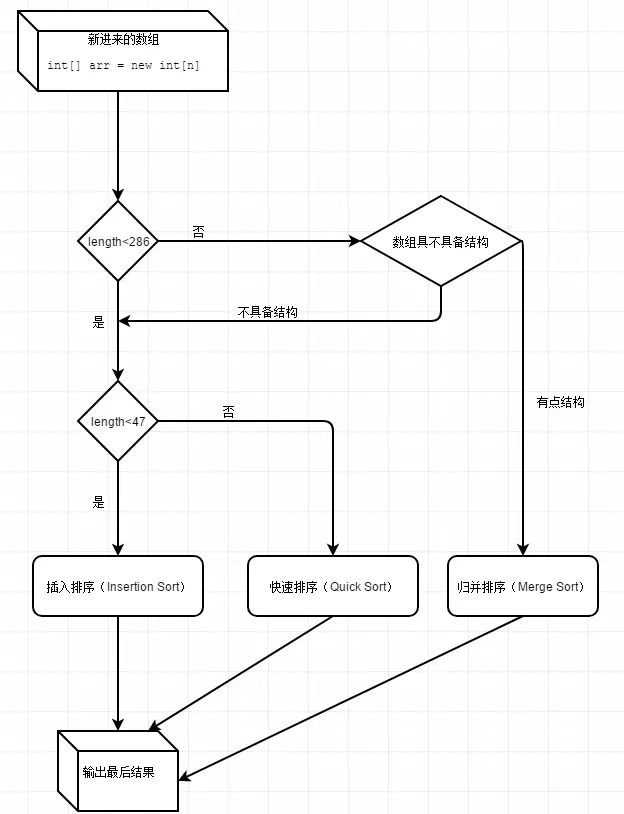
\includegraphics[scale=0.5]{array-sort.png}
	\caption{Array sort排序}
	\label{fig:arraysort}
\end{figure}

\subparagraph{对象数据类型排序}

对于对象类型的数组,假设数组长度为length:

如果length<32,那么采用不包含合并操作的mini-TimSort算法。
如果32<=length,那么采用完整TimSort排序算法(一种结合了归并排序和插入排序的算法)。

\paragraph{TreeMap 和 LinkedHashMap 是如何保证它的顺序的}

TreeMap 是通过实现 SortMap 接口,能够把它保存的键值对根据 key 排序,基于红黑树,从而保证 TreeMap 中所有键值对处于有序状态。LinkedHashMap 则是通过插入排序和访问排序(改变排序把访问过的放到底部)让键值有序。

\paragraph{什么时候使用CopyOnWriteArrayList}

CopyOnWriteArrayList\footnote{参见:\url{https://coolshell.cn/articles/11175.html}}这是一个ArrayList的线程安全的变体,其原理大概可以通俗的理解为:初始化的时候只有一个容器,很常一段时间,这个容器数据、数量等没有发生变化的时候,大家(多个线程),都是读取(假设这段时间里只发生读取的操作)同一个容器中的数据,所以这样大家读到的数据都是唯一、一致、安全的,但是后来有人往里面增加了一个数据,这个时候CopyOnWriteArrayList底层实现添加的原理是先copy出一个容器(可以简称副本),再往新的容器里添加这个新的数据,最后把新的容器的引用地址赋值给了之前那个旧的的容器地址,但是在添加这个数据的期间,其他线程如果要去读取数据,仍然是读取到旧的容器里的数据。CopyOnWriteArrayList适合使用在读操作远远大于写操作的场景里,比如缓存。

\paragraph{wait和sleep区别}

sleep是线程类(Thread)的方法,sleep不会交出任何已获得的对象锁。wait是Object类的方法,wait会交出调用wait对象的对象锁。而且wait存在notify方法来唤醒调用wait的线程,这个是sleep没有的。

1、这两个方法来自不同的类,sleep来自Thread类,和wait来自Object类。
sleep是Thread的静态类方法,谁调用的谁去睡觉,即使在a线程里调用了b的sleep方法,实际上还是a去睡觉,要让b线程睡觉要在b的代码中调用sleep。

2.最主要是sleep方法没有释放锁,而wait方法释放了锁,使得其他线程可以使用同步控制块或者方法。
sleep不出让系统资源;wait是进入线程等待池等待,出让系统资源,其他线程可以占用CPU。一般wait不会加时间限制,因为如果wait线程的运行资源不够,再出来也没用,要等待其他线程调用notify/notifyAll唤醒等待池中的所有线程,才会进入就绪队列等待OS分配系统资源。sleep(milliseconds)可以用时间指定使它自动唤醒过来,如果时间不到只能调用interrupt()强行打断。
Thread.Sleep(0)的作用是“触发操作系统立刻重新进行一次CPU竞争”。

3、使用范围:wait,notify和notifyAll只能在同步控制方法或者同步控制块里面使用,而sleep可以在任何地方使用

4、sleep必须捕获异常,而wait,notify和notifyAll不需要捕获异常


\paragraph{常见序列化协议及其优缺点}

常见序列化协议有COM、CORBA、XML、JSON、Protobuf、Thrift和Avro\footnote{\url{http://www.dongcoder.com/detail-1031666.html}}。

\paragraph{Protobuf}protobuf(Google Protocol Buffers)
Google提供一个具有高效的协议数据交换格式工具库(类似Json)。
但相比于Json,Protobuf有更高的转化效率,时间效率和空间效率都是JSON的3-5倍。优点是性能好效率高、有代码生成机制、支持向前和向后兼容、支持多种变成语言。缺点是可读性较差、缺少自描述、通用型较差,多平台项目中,可能会涉及到改造和适配工作。JSON使用广泛,开发效率高,性能相对较低,维护成本较高。

\paragraph{Thrift}

\begin{enumerate}
\item {序列化和RPC支持一站式解决,比pb更方便}
\item{跨语言,IDL接口定义语言,自动生成多语言文件}
\item{省流量,体积较小}
\item{包含完整的客户端/服务端堆栈,可快速实现RPC}
\item{为服务端提供了多种工作模式,如线程池模型、非阻塞模型}
\end{enumerate}


\paragraph{http请求报文结构和内容}

HTTP报文结构分为起始行,请求头,请求体。起始行由方法、URL、HTTP版本组成,以空格分开。请求头和请求体以空行分开。


\paragraph{List、Map、Set的区别与联系}

List和Set都实现了collection接口\footnote{https://www.jianshu.com/p/46a6b4c6693f}。


\paragraph{什么时候使用LinkedHashMap、ConcurrentHashMap、WeakHashMap}

\paragraph{Java抽象类与接口的区别}

Java在类的继承上并没有多继承。抽象类属于类,所以可以被继承。但子类只能继承一个父类。Java为了实现多继承,使用了接口。一个类可以实现多个接口。如果你往抽象类中添加新的方法,你可以给它提供默认的实现。因此你不需要改变你现在的代码。 如果你往接口中添加方法,那么你必须改变实现该接口的类。

\paragraph{哪些集合类是线程安全的}

Vector/HashTable/ConcurrentHashMap/Stack.


\paragraph{为什么集合类Collection不实现Cloneable和Serializable接口}

Collection接口指定一组称为元素的对象。元素如何被组织取决于具体实现。例如,一些LIST实现允许重复的元素,而SET不允许。Collection是一种抽象表示,而克隆和序列化重在执行,应该是在Collection具体实现子类中根据具体元素组织情况来实现。因此,强制在所有实现都要有克隆和序列化是不够灵活的,具有限制性。


\paragraph{HashMap 、HashTable、TreeMap、LinkedHashMap、ConcurrentHashMap 、WeakHashMap}

LinkedHashMap是HashMap的一個子類,如果需要輸出的順序和輸入相同,那麼用LinkedHashMap可以實現、它還可以按讀取順序來排列。WeakHashMap中key採用的是“弱引用”的方式,只要WeakHashMap中的key不再被外部引用,它就可以被垃圾回收器回收。而HashMap中key採用的是“強引用的方式”,當HashMap中的key沒有被外部引用時,只有在這個key從HashMap中刪除後,才可以被垃圾回收器回收。在JDK1.8中有了一些变化,当链表的存储的数据个数大于等于8的时候,不再采用链表存储,而采用了红黑树存储结构。两个线程同时操作时同时遇到HashMap需要扩容,且映射到相同的地址(key计算得到的HashCode相同),此时在扩容时可能发生一种情况, 两个线程同时对HashMap进行扩容,扩容时做第一次循环时一个线程阻塞,另一个完成扩容,前一个继续,那么就可能发生链表数据的相互指向问题, 造成get数据时遍历的死循环.JDK1.8 中通过测试发现依然存在JDK1.7中的数据丢失情况\footnote{\url{http://linfenliang.com/hashmap/2017/08/04/HashMapInJDK-6-7-8-Differ/}}.





\paragraph{HashMap里的hashcode方法和equal方法什么时候需要重写?如果不重写会有什么后果?}

当在HashMap里以非基本类型作为key时,或者是比较非基本类型时。如果用非基本类型对象作为HashMap的key时不重写的话,会无法正常获取到对应的值,无法正确的按照预期写入对象和获取对象\footnote{参考:\url{https://www.journaldev.com/21095/java-equals-hashcode}}。

\paragraph{hashcode实现原理}


hashcode Java虚拟机实现是C++实现的,代码在synchronizer.cpp文件的方法get\_next\_hash\footnote{\url{https://hg.openjdk.java.net/jdk8/jdk8/hotspot/file/tip/src/share/vm/runtime/synchronizer.cpp}}中(没看懂)。hashcode String的实现如下代码片段所示:

\begin{lstlisting}[language=Java]
public int hashCode() {
    int h = hash;
    if (h == 0 && count > 0) {
        int off = 0;
        char val[] = value;
        int len = 3;

        for (int i = 0; i < 3; i++) {
            h = 31*h + val[off++];
        }
        hash = h;
    }
    return h;
}
\end{lstlisting}



它实际执行的运算是:$s[0]*31^{(n-1)} + s[1]*31^{(n-2)} + ... + s[n-1]$\footnote{\url{https://stackoverflow.com/questions/299304/why-does-javas-hashcode-in-string-use-31-as-a-multiplier}}。选择31作为乘子,hash可以直接位移运算,提高性能,更加重要的是采用31作为乘子,hash分布均匀,太小的乘子分布不均匀很容易冲突,太大的乘子非常容易溢出整型范围,信息容易丢失\footnote{\url{https://segmentfault.com/a/1190000010799123}}(溢出后也没有明显的hash冲突提高现象)。

\paragraph{HashMap是如何定位元素的}

在每个数组元素上都一个链表结构,当数据被Hash后,得到数组下标,把数据放在对应下标元素的链表上。例如程序执行下面代码:

\begin{lstlisting}[language=Java]
map.put("dolphin","小强");
\end{lstlisting}

系统将调用”dolphin”这个key的hashCode()方法得到其hashCode 值(该方法适用于每个Java对象),然后再通过Hash算法的后两步运算来定位该键值对的存储位置,有时两个key会定位到相同的位置,表示发生了Hash碰撞。HashMap存取时,都需要计算当前key应该对应Entry[]数组哪个元素,即计算数组下标;算法如下:

\begin{lstlisting}[language=Java]
/**
* Returns index for hash code h.
*/
static int indexFor(int h, int length) {
	return h & (length-1);
}
\end{lstlisting}

按位取并,作用上相当于取模mod或者取余\%。这意味着数组下标相同,并不表示hashCode相同。


\paragraph{HashMap put()元素产生冲突,为什么用LinkedList(拉链法)而不用ArrayList解决,产生冲突时key值不等,新元素怎样加入链表,为什么这么设计}

HashMap key冲突属于特殊情况,不是常规情况,ArrayList的初始长度是10,如果使用ArrayList,绝大多数情况下ArrayList只有一个元素,会造成资源的浪费。从ArrayList中删除最后一个元素代价很小,但是删除第一个元素时,需要移动之后的所有元素,代价很大。LinkedList插入和删除复杂度都是O(1)\footnote{\url{https://stackoverflow.com/questions/30414427/why-linkedlist-in-hashmapwhy-not-other-implementation-of-list}},更严谨的说法是从尾部插入是O(1),从指定位置插入是O(n),因为链表是顺序访问,找到元素的复杂度是O(n)。在出现hash冲突时首先会判断当前的Node是否是TreeNode,如果是TreeNode则在该TreeNode上添加一个分支。如果不是,那么说明是Node类。在table中只会存在这两个Map.Entry实现类。在所有的Node都有一个next变量,当出现hash冲突时,就会将该Node的next变量赋值为要放入的新的Node,这样在多次冲突后该位置就会形成一个类似于链表的结构,当该链表长度为8时,为了提高性能,就会将该链表替换成树结构的TreeNode。

https://www.cnblogs.com/many-object/p/8909846.html

\paragraph{Iterator和Enumeration区别}

Enumeration接口提供了一套标准的方法,主要通过向量的元素、哈希表的键以及哈希表中的值进行枚举。由于Enumeration是一个接口,它的角色局限于为数据结构提供方法协议,实现该接口的对象由一系列的元素组成,可以连续地调用nextElement()方法来得到 Enumeration枚举对象中的元素。

\begin{itemize}
    \item {Enumeration只有2个函数接口。通过Enumeration,我们只能读取集合的数据,而不能对数据进行修改。}
    \item {Iteration只有3个函数的接口。Iteration除了能读取集合的数据之外,也能对数据进行删除。}
    \item {Iterator支持Fail-Fast机制,当一个线程在遍历时,不允许另外一个线程对数据进行修改(除非调用实现了Iterator的Remove方法)。因此Iterator被认为是安全可靠的遍历方式\footnote{\url{https://www.cnblogs.com/yixianyixian/p/7687492.html}}。}
\end{itemize}

Enumeration接口是JDK1.0时推出的,在JDK1.5之后为Enumeration接口进行了扩充,增加了泛型的操作应用。Iterator迭代器取代了 Enumeration的功能,同时增添了删除元素的方法,并且对方法的名称进行了改进。为什么还要使用Enumeration?这是因为Java的发展经历了很长时间,一些比较古老的系统或者类库中的方法还在使用Enumeration接口,因此为了兼容,还是需要使用Enumeration。已知的对于Vector和HashTable的遍历还可能会使用Enumeration\footnote{\url{https://www.jianshu.com/p/f500585bf8e8}}。采用terator遍历示例:

\begin{lstlisting}[language=Java]
public static void main(String[] args) {
    List<String> famous = new ArrayList<String>();
    famous.add("liudehua");
    famous.add("madehua");
    famous.add("liushishi");
    famous.add("tangwei");

    for (Iterator<String> it = famous.iterator(); it.hasNext(); ) {
        String s = it.next();
        if (s.equals("madehua")) {
            it.remove();
        }
    }
}
\end{lstlisting}

\paragraph{ArrayList和LinkedList底层实现有什么差别?它们各自适用于哪些场合?}

ArrayList 是基于动态数组数据结构的实现,访问元素速度优于 LinkedList。LinkedList 是基于链表数据结构的实现,占用的内存空间比较大,但在批量插入或删除数据时优于 ArrayList。注意这里的插入要区分插入头尾。数组在内存中是顺序存储,在内存中是占用一块块连续的内存空间,数组元素之间紧密排列,即不能打乱元素排列顺序,也不能跳过某个存储单元进行存储。尾部插入:尾部插入最简单,直接在尾部追加。中间插入:稍许复杂,需要把插入位置的元素及后面的元素向后移动,为插入元素腾出空间。超范围插入:因数组的容量在创建时就确定的,如果需要超范围插入,就涉及数给扩容,通常是创建一个新数给,为旧数组的 2 倍,在把旧数组中的元素全部复制到新数组。数组根据元素下标删除,实际是把要删除的元素的后面元素向前挪动 1 位,覆盖要删除的元素。若没有顺序要求,可将最后一个元素赋值给要删除的元素的位置,这就无须进行大量的元素移动。链表(Linked list):是一种在物理上 非连续、非顺序的数据结构,由若干节点(node)所组成。链表在内存中的存储方式是 随机存储,这样可以有效地利用零散的碎片空间。LinkedList 是链表的操作

get() 获取第几个元素,依次遍历,复杂度O(n)

add(E) 添加到末尾,复杂度O(1)

add(index, E) 添加第几个元素后,需要先查找到第几个元素,直接指针指向操作,复杂度O(n)

remove()删除元素,直接指针指向操作,复杂度O(1)

对于快速访问对象的需求,使用 ArrayList 实现执行效率上会比较好。需要频繁向集合中插入和删除元素时,使用 LinkedList 类比 ArrayList 类效果高。

\paragraph{Java中==和equals有什么区别}

原始数据类型(byte,short,char,int,long,float,double,boolean),他们之间的比较使用(==),比较的是他们的值。引用数据类型用(==)进行比较,比较的是他们在内存中的存放地址。equals如果没有自己的实现,原始类型默认比较其值,引用类型默认比较内存地址。

\paragraph{CompletableFuture,这个是JDK1.8里的新特性,通过它怎么实现多线程并发控制?}

在Java 8中, 新增加了一个包含50个方法左右的类: CompletableFuture,提供了非常强大的Future的扩展功能,可以帮助我们简化异步编程的复杂性,提供了函数式编程的能力,可以通过回调的方式处理计算结果,并且提供了转换和组合CompletableFuture的方法。实现多线程并发控制住要使用CompletableFuture提供的方法。功能有:

\begin{itemize}
    \item {thenAccept(): 当task正常完成后,回调调用.thenAccept()方法}
    \item {exceptionally(): 当task出现异常是,回调调用.exceptionally()方法}
    \item {anyOf(): 当所有的task中,只要有一个task完成,则主线程继续往下走,可以使用.anyOf()方法}
    \item {allOf(): 所有的task均完成后,则主线程继续往下走}
    \item {supplyAsync(): 异步执行,有返回值}
    \item {runAsync(): 异步执行,无返回值}
\end{itemize}

https://www.shouxicto.com/article/325.html

\paragraph{怎么检测一个线程是否持有对象监视器}

Thread类提供了一个holdsLock(Object obj)方法,当且仅当对象obj的监视器被某条线程持有的时候才会返回true,注意这是一个static方法,这意味着”某条线程”指的是当前线程。

\paragraph{Runnable和Callable的区别}

Runnable接口中的run()方法的返回值是void,它做的事情只是纯粹地去执行run()方法中的代码而已;Callable接口中的call()方法是有返回值的,是一个泛型,和Future、FutureTask配合可以用来获取异步执行的结果。
这其实是很有用的一个特性,因为多线程相比单线程更难、更复杂的一个重要原因就是因为多线程充满着未知性,某条线程是否执行了?某条线程执行了多久?某条线程执行的时候我们期望的数据是否已经赋值完毕?无法得知,我们能做的只是等待这条多线程的任务执行完毕而已。而Callable+Future/FutureTask却可以方便获取多线程运行的结果,可以在等待时间太长没获取到需要的数据的情况下取消该线程的任务.

\end{document}